\section{Preventivo}

La sezione Preventivo ha lo scopo di redigere un preventivo sul costo orario per ogni ora di lavoro svolta dai membri del gruppo, in questo modo possiamo stimare il budget necessario per la realizzazione del progetto. \\
La suddivisione oraria segue alcune regole comuni per ogni membro:
\begin{itemize}
	\item I componenti dovranno svolgere tutti i ruoli almeno una volta;
	\item Ogni componente dovrà lavorare almeno 8 ore per ogni ruolo;
	\item Tutti i componenti avranno lo stesso numero ore di lavoro ad ogni revisione.
\end{itemize}
Le sigle per i vari ruoli sono:
\begin{itemize}
	\item RE: Responsabile;
	\item AM: Amministratore;
	\item AN: Analista;
	\item PJ: Progettista;
	\item PR: Programmatore;
	\item VE: Verificatore.
\end{itemize}

\newpage
\subsection{Avvio ed analisi dei requisiti}
\subsubsection{Prospetto orario}

Nel periodo di Avvio ed analisi dei requisiti la suddivisione oraria, per ogni membro del gruppo, è la seguente:

\begin{longtable}{|C{.30\textwidth}|C{.06\textwidth}|C{.06\textwidth}|C{.06\textwidth} | C{.06\textwidth}| C{.06\textwidth} | C{.06\textwidth} | C{.10\textwidth} |}
\hline
\textbf{Nome} & \textbf{RE} & \textbf{AM} & \textbf{AN} & \textbf{PJ} & \textbf{PR} & \textbf{VE} & \textbf{Totale}\\
\hline 
Marco Chilese & - & - & 10 & - & - & 15 & 25 \\
\hline
Marco Favaro & - & - & 14 & - & - & 11 & 25 \\
\hline
Diego Mazzalovo & - & - & 18 & - & - & 7 & 25 \\
\hline
Carlotta Segna & 11 & - & 5 & - & - & 9 & 25 \\
\hline
Matteo Slanzi & - & 8 & 10 & - & - & 7 & 25 \\
\hline
Bogdan Stanciu & 15 & - & 7 & - & - & 3 & 25\\
\hline
Luca Violato & - & 15 & 5 & - & - & 5 & 25 \\
\hline


\caption{Distribuzione oraria del periodo di Avvio ed analisi dei requisiti}
\label{Distribuzione oraria del periodo di Avvio ed analisi dei requisiti}
\end{longtable}

Il seguente grafico dà una visione grafica della suddivisione dei ruoli per il periodo di Avvio ed analisi dei requisiti:

\begin{figure}[h]
	\centering
  		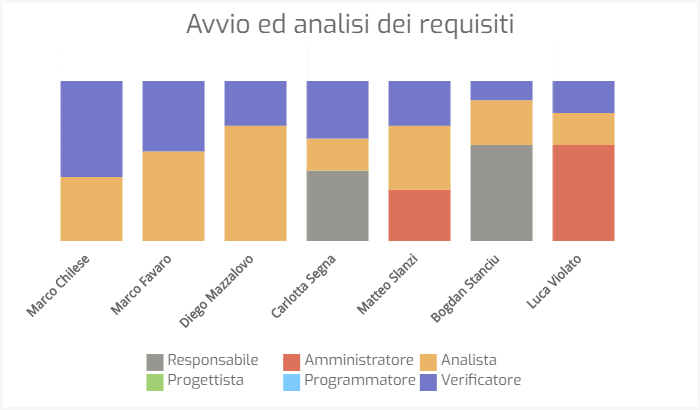
\includegraphics[width=1\linewidth]{./images/avvio_analisi_requisiti.png}
  		\caption{Grafico suddivisione ore per persona nel periodo di Avvio ed analisi dei requisiti}
  		\label{fig:grafico suddivione ruoli periodo di Avvio ed analisi requisiti}
\end{figure}



\subsubsection{Prospetto economico}
Nel periodo di Avvio ed analisi dei requisiti la suddivisione oraria, per quanto riguarda i ruoli, è la seguente: 

\begin{longtable}{| C{.30\textwidth}| C{.15\textwidth}| C{.20\textwidth}|}
\hline
\textbf{Ruolo} & \textbf{Ore} & \textbf{Costo in \euro} \\
\hline
Responsabile & 26 & \EUR{780.00} \\
\hline
Amministratore & 23 & \EUR{460.00} \\
\hline
Analista & 69 & \EUR{1725.00} \\
\hline
Progettista & - & - \\
\hline
Programmatore & - & - \\
\hline
Verificatore & 57 & \EUR{855.00}\\
\hline
\textbf{Totale} & 175 & \EUR{3820.00} \\
\hline

\caption{Distribuzione oraria del periodo di Avvio ed analisi dei requisiti}
\label{tabella distribuzione oraria del periodo di Avvio ed analisi dei requisiti}
\end{longtable}

Il seguente grafico dà una rappresentazione visiva della suddivisione nei ruoli:
\begin{figure}[H]
	\centering
  		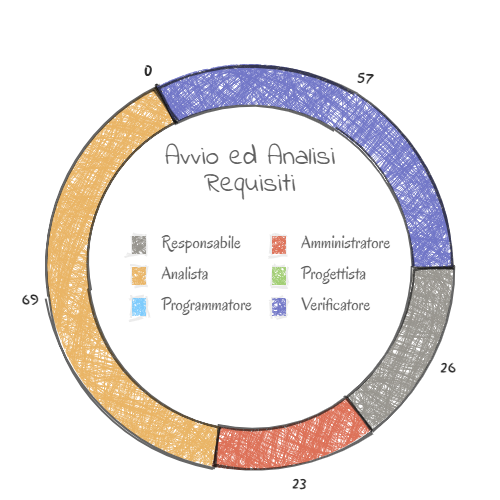
\includegraphics[width=0.8\linewidth]{./images/torta_aar.png}
  		\caption{Grafico suddivisione ore per persona nel periodo di Avvio ed analisi dei requisiti}
  		\label{fig:grafico suddivione ruoli periodo di Avvio ed analisi dei requisiti}
\end{figure}

\subsection{Risanamento criticità}
\subsubsection{Prospetto orario}

Nel periodo di Risanamento criticità la suddivisione oraria, per quanto riguarda i ruoli, è la seguente:

\begin{longtable}{|C{.30\textwidth}|C{.06\textwidth}|C{.06\textwidth}|C{.06\textwidth} | C{.06\textwidth}| C{.06\textwidth} | C{.06\textwidth} | C{.10\textwidth} |}
\hline
\textbf{Nome} & \textbf{RE} & \textbf{AM} & \textbf{AN} & \textbf{PJ} & \textbf{PR} & \textbf{VE} & \textbf{Totale}\\
\hline 
Marco Chilese & - & - & - & - & - & 7 & 7 \\
\hline
Marco Favaro & - & - & 7 & - & - & - & 7 \\
\hline
Diego Mazzalovo & - & - & 7 & - & - & - & 7 \\
\hline
Carlotta Segna & - & - & - & - & - & 7 & 7 \\
\hline
Matteo Slanzi & - & - & 7 & - & - & - & 7 \\
\hline
Bogdan Stanciu & 7 & - & - & - & - & 0 & 7 \\
\hline
Luca Violato & - & 7 & - & - & - & - & 7 \\
\hline

\caption{Distribuzione oraria del periodo di Risanamento criticità}
\label{Distribuzione oraria del periodo di Risanamento criticità}
\end{longtable}



Il seguente grafico dà una visione grafica della suddivisione dei ruoli per il periodo di Risanamento criticità:
\begin{figure}[H]
  \centering
  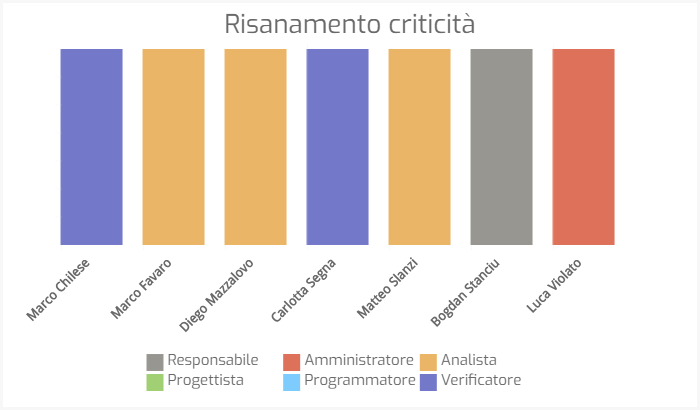
\includegraphics[width=1\linewidth]{./images/risanemento_criticita1.png}
  \caption{Grafico suddivisione ore nei ruoli nel periodo di Risanamento criticità}
  \label{fig:grafico suddivione ruoli nel periodo di Risanamento criticità}
\end{figure}

\subsubsection{Prospetto economico}
\begin{longtable}{| C{.30\textwidth}| C{.15\textwidth}| C{.20\textwidth}|}
\hline
\textbf{Ruolo} & \textbf{Ore} & \textbf{Costo in \euro} \\
\hline 
Responsabile & 7 & \EUR{210.00} \\
\hline
Amministratore & 7 & \EUR{140.00} \\
\hline
Analista & 21 & \EUR{525.00} \\
\hline
Progettista & - & - \\
\hline
Programmatore & - & - \\
\hline
Verificatore & 14 & \EUR{210.00}\\
\hline
\textbf{Totale} & 49 & \EUR{1085.00} \\
\hline


\caption{Distribuzione oraria del periodo di Risanamento criticità}
\label{Distribuzione oraria del periodo di Risanamento criticità}
\end{longtable}

Il seguente grafico dà una rappresentazione visiva della suddivisione nei ruoli:
\begin{figure}[H]
	\centering
  		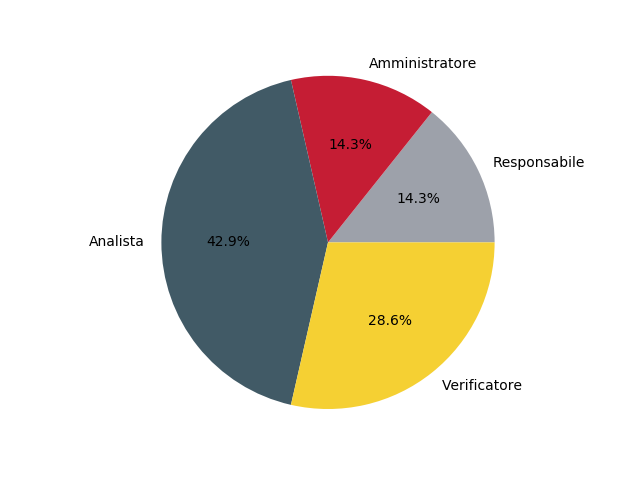
\includegraphics[width=0.8\linewidth]{./images/torta_rc1.png}
  		\caption{Grafico suddivisione ore per persona nel periodo di Risanamento criticità}
  		\label{fig:grafico suddivione ruoli periodo di Risanamento criticità}
\end{figure}


\subsection{Progettazione architetturale}
\subsubsection{Prospetto orario}

Nel periodo di Progettazione architetturale la suddivisione oraria, per ogni membro del gruppo, è la seguente:


\begin{longtable}{|C{.30\textwidth}|C{.06\textwidth}|C{.06\textwidth}|C{.06\textwidth} | C{.06\textwidth}| C{.06\textwidth} | C{.06\textwidth} | C{.10\textwidth} |}
\hline
\textbf{Nome} & \textbf{RE} & \textbf{AM} & \textbf{AN} & \textbf{PJ} & \textbf{PR} & \textbf{VE} & \textbf{Totale}\\
\hline 
Marco Chilese & - & 10 & - & 8 & 7 & - & 25 \\
\hline
Marco Favaro & 10 & - & 8 & - & - & 7 & 25 \\
\hline
Diego Mazzalovo & 8 & - & - & 10 & 7 & - & 25 \\ 
\hline
Carlotta Segna & - & - & 5 & 5 & 15 & - & 25 \\
\hline
Matteo Slanzi & - & - & 5 & - & 8 & 12 & 25 \\
\hline
Bogdan Stanciu & - & 8 & - & - & 17 & - & 25 \\
\hline
Luca Violato & - & - & 7 & 8 & - & 10 & 25 \\
\hline 

\caption{Distribuzione oraria del periodo di Progettazione architetturale}
\label{Distribuzione oraria del periodo di Progettazione architetturale}
\end{longtable}

Il seguente grafico dà una visione grafica della suddivisione dei ruoli per il periodo di Avvio ed analisi dei requisiti:

\begin{figure}[H]
	\centering
  		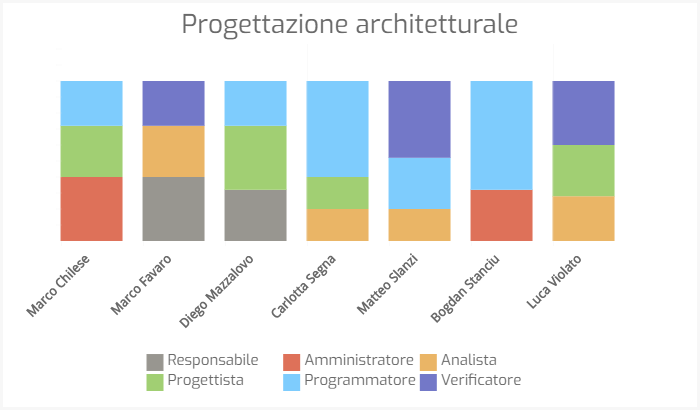
\includegraphics[width=1\linewidth]{./images/progettazione_architetturale.png}
  		\caption{Grafico suddivisione ore per persona nel periodo di Progettazione architetturale}
  		\label{fig:grafico suddivione ruoli periodo di Progettazione architetturale}
\end{figure}



\subsubsection{Prospetto economico}
\begin{longtable}{| C{.30\textwidth}| C{.15\textwidth}| C{.20\textwidth}|}
\hline
\textbf{Ruolo} & \textbf{Ore} & \textbf{Costo in \euro} \\
\hline 
Responsabile & 18 & \EUR{540.00} \\
\hline
Amministratore & 18 & \EUR{360.00}\\
\hline
Analista & 25 & \EUR{625.00} \\
\hline
Progettista & 31 & \EUR{682.00} \\
\hline
Programmatore & 54 & \EUR{810.00} \\
\hline
Verificatore & 29 & \EUR{435.00} \\
\hline
\textbf{Totale} & 175 & \EUR{3452.00}\\ 
\hline

\caption{Distribuzione oraria del periodo di Progettazione architetturale}
\label{Distribuzione oraria del periodo di Progettazione architetturale}
\end{longtable}

Il seguente grafico dà una rappresentazione visiva della suddivisione nei ruoli:
\begin{figure}[H]
	\centering
  		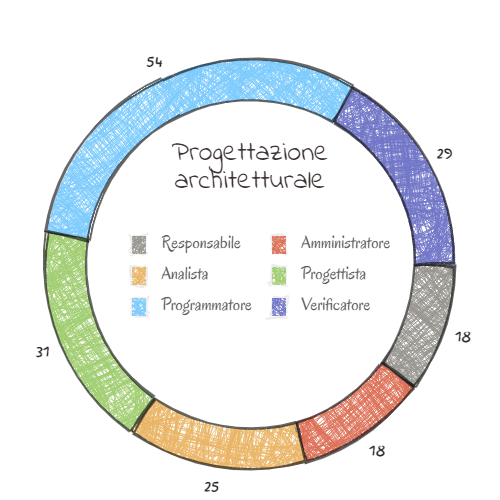
\includegraphics[width=0.8\linewidth]{./images/torta_pa.png}
  		\caption{Grafico suddivisione ore per persona nel periodo di Progettazione architetturale}
  		\label{fig:grafico suddivione ruoli periodo di Progettazione architetturale}
\end{figure}


\subsection{Risanamento criticità}
\subsubsection{Prospetto orario}

\begin{longtable}{|C{.30\textwidth}|C{.06\textwidth}|C{.06\textwidth}|C{.06\textwidth} | C{.06\textwidth}| C{.06\textwidth} | C{.06\textwidth} | C{.10\textwidth} |}
\hline
\textbf{Nome} & \textbf{RE} & \textbf{AM} & \textbf{AN} & \textbf{PJ} & \textbf{PR} & \textbf{VE} & \textbf{Totale}\\
\hline 
Marco Chilese & - & 6 & - & - & - & - & 6 \\
\hline
Marco Favaro & 6 - & - & - & - & - & - & 6 \\
\hline
Diego Mazzalovo & - & - & - & 6 & - & - & 6 \\
\hline
Carlotta Segna & - & - & - & - & 6 & - & 6 \\
\hline
Matteo Slanzi & - & - & - & - & - & 6 & 6 \\
\hline
Bogdan Stanciu & - & - & 6 & - & - & - & 6 \\
\hline
Luca Violato & - & - & - & - & - & 6 & 6 \\   
\hline


\caption{Distribuzione oraria del periodo di Risanamento criticità}
\label{Distribuzione oraria del periodo di Risanamento criticità}
\end{longtable}

Il seguente grafico dà una visione grafica della suddivisione dei ruoli per il periodo di Risanamento criticità:\begin{figure}[H]
	\centering
  		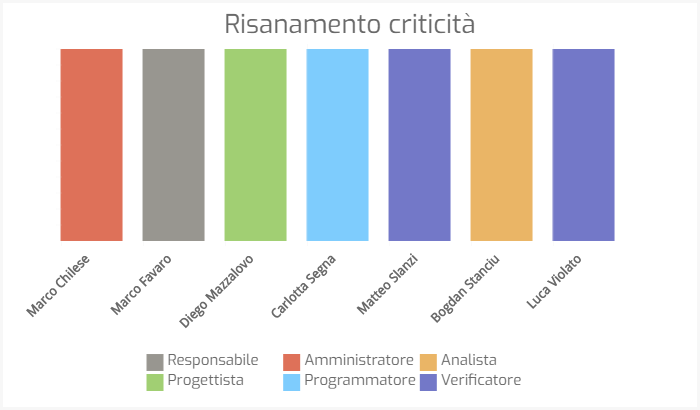
\includegraphics[width=1\linewidth]{./images/risanamento_criticita2.png}
  		\caption{Grafico suddivisione ore nei ruoli nel periodo di Risanamento criticità}
  		\label{fig:grafico suddivione ruoli nel periodo di Risanamento criticità}
\end{figure}



\subsubsection{Prospetto economico}
\begin{longtable}{| C{.30\textwidth}| C{.15\textwidth}| C{.20\textwidth}|}
\hline
\textbf{Ruolo} & \textbf{Ore} & \textbf{Costo in \euro} \\
\hline 
Responsabile & 6 & \EUR{180.00} \\
\hline
Amministratore & 6 & \EUR{120.00} \\
\hline
Analista & 6 & \EUR{150.00} \\
\hline
Progettista & 6 & \EUR{132.00}\\
\hline
Programmatore & 6 & \EUR{90.00} \\
\hline 
Verificatore & 12 & \EUR{180.00} \\
\hline
\textbf{Totale} & 42 & \EUR{852.00} \\
\hline 

\caption{Distribuzione oraria del periodo di Risanamento criticità}
\label{Distribuzione oraria del periodo di Risanamento criticità}
\end{longtable}

Il seguente grafico dà una rappresentazione visiva della suddivisione nei ruoli:
\begin{figure}[H]
	\centering
  		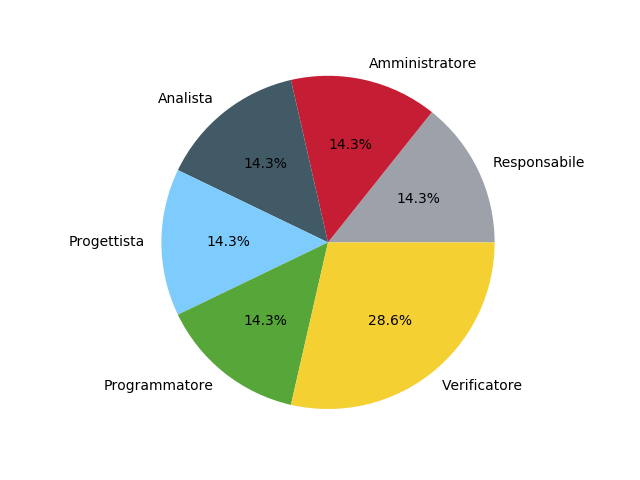
\includegraphics[width=0.8\linewidth]{./images/torta_rc2.png}
  		\caption{Grafico suddivisione ore per persona nel periodo di Risanamento criticità}
  		\label{fig:grafico suddivione ruoli periodo di Risanamento criticità}
\end{figure}

\newpage
\subsection{Progettazione di dettaglio e codifica}
\subsubsection{Prospetto orario}

Nel periodo di Progettazione di dettaglio e codifica la suddivisione oraria, per ogni membro del gruppo, è la seguente:

\begin{longtable}{|C{.30\textwidth}|C{.06\textwidth}|C{.06\textwidth}|C{.06\textwidth} | C{.06\textwidth}| C{.06\textwidth} | C{.06\textwidth} | C{.10\textwidth} |}
	\hline
	\textbf{Nome} & \textbf{RE} & \textbf{AM} & \textbf{AN} & \textbf{PJ} & \textbf{PR} & \textbf{VE} & \textbf{Totale}\\
	\hline 
	Marco Chilese & - & - & 8 & 17 & 18 & 12 & 55 \\
	\hline
	Marco Favaro &  - & - & - & 15 & 21 & 19 & 55 \\
	\hline
	Diego Mazzalovo & - & 8 & - & 12 & 22 & 13 & 55 \\
	\hline
	Carlotta Segna & - & 8 & - & 15 & 18 & 14 & 55 \\
	\hline
	Matteo Slanzi & 10 & - & 5 & 20 & 20 & - & 55 \\
	\hline
	Bogdan Stanciu & - & - & 11 & 24 & - & 20 & 55 \\
	\hline
	Luca Violato & 10 & - & - & 15 & 21 & 9 & 55 \\   
	\hline


\caption{Distribuzione oraria del periodo di Progettazione di dettaglio e codifica}
\label{Distribuzione oraria del periodo di Progettazione di dettaglio e codifica}
\end{longtable}

Il seguente grafico dà una visione grafica della suddivisione dei ruoli per il periodo di Progettazione di dettaglio e codifica:

\begin{figure}[H]
	\centering
	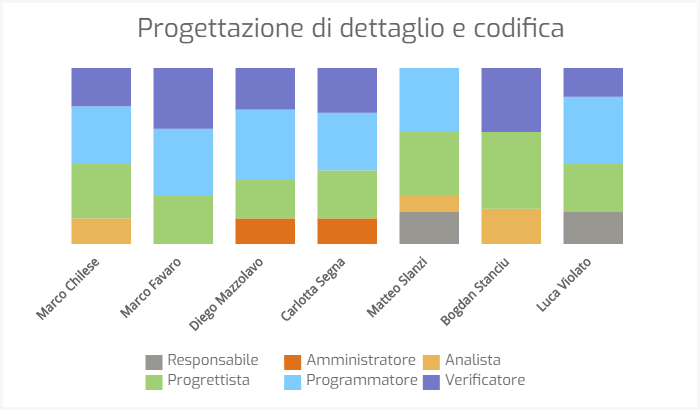
\includegraphics[width=1\linewidth]{./images/Bar_progettazione_dettaglio_codifica.png}
	\caption{Grafico suddivisione ore per persona nel periodo di Progettazione  dettaglio e codifica}
	\label{fig:grafico suddivione ruoli periodo di Progettazione di dettaglio e codifica}
\end{figure}

\subsubsection{Prospetto economico}
\begin{longtable}{| C{.30\textwidth}| C{.15\textwidth}| C{.20\textwidth}|}
	\hline
	\textbf{Ruolo} & \textbf{Ore} & \textbf{Costo in \euro} \\
	\hline 
	Responsabile & 20 & \EUR{600.00} \\
	\hline
	Amministratore & 16 & \EUR{320.00}\\
	\hline
	Analista & 24 & \EUR{600.00} \\
	\hline
	Progettista & 118 & \EUR{2596.00} \\
	\hline
	Programmatore & 120 & \EUR{1800.00} \\
	\hline
	Verificatore & 87 & \EUR{1305.00} \\
	\hline
	\textbf{Totale} & 385 & \EUR{7221.00}\\ 
	\hline
	
	\caption{Distribuzione oraria del periodo di Progettazione di dettaglio e codifica}
	\label{Distribuzione oraria del periodo di Progettazione di dettaglio e codifica}
\end{longtable}

Il seguente grafico dà una rappresentazione visiva della suddivisione nei ruoli:
\begin{figure}[H]
	\centering
	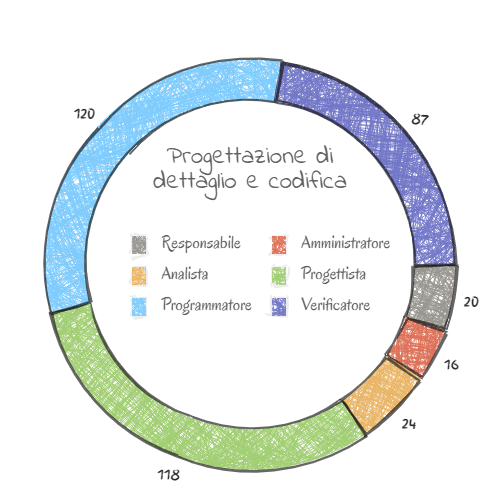
\includegraphics[width=0.8\linewidth]{./images/Torta_progettazione_dettaglioCod.png}
	\caption{Grafico suddivisione ore per persona nel periodo di Progettazione  di dettaglio e codifica}
	\label{fig:grafico suddivione ruoli periodo di Progettazione  di dettaglio e codifica}
\end{figure}


\subsection{Risanamento criticità}
\subsubsection{Prospetto orario}
\begin{longtable}{|C{.30\textwidth}|C{.06\textwidth}|C{.06\textwidth}|C{.06\textwidth} | C{.06\textwidth}| C{.06\textwidth} | C{.06\textwidth} | C{.10\textwidth} |}
	\hline
	\textbf{Nome} & \textbf{RE} & \textbf{AM} & \textbf{AN} & \textbf{PJ} & \textbf{PR} & \textbf{VE} & \textbf{Totale}\\
	\hline 
	Marco Chilese & - & - & 5 & - & - & - & 5 \\
	\hline
	Marco Favaro & - & - & - & - & - & 5 & 5 \\
	\hline
	Diego Mazzalovo & - & - & - & - & 5 & - & 5 \\
	\hline
	Carlotta Segna & - & 5 & - & - & - & - & 5 \\
	\hline
	Matteo Slanzi & - & - & - & - & - & 5 & 5 \\
	\hline
	Bogdan Stanciu & - & - & - & - & 5 & - & 5 \\
	\hline
	Luca Violato & 5 & - & - & - & - & - & 5 \\   
	\hline
	
	
	\caption{Distribuzione oraria del periodo di Risanamento criticità}
	\label{Distribuzione oraria del periodo di Risanamento criticità}
\end{longtable}

Il seguente grafico dà una visione grafica della suddivisione dei ruoli per il periodo di Risanamento criticità:\begin{figure}[H]
	\centering
	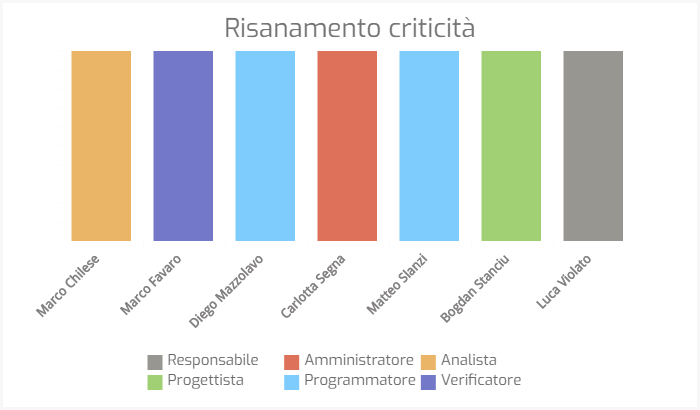
\includegraphics[width=1\linewidth]{./images/Bar_risanamento_criticita3.png}
	\caption{Grafico suddivisione ore nei ruoli nel periodo di Risanamento criticità}
	\label{fig:grafico suddivione ruoli nel periodo di Risanamento criticità}
\end{figure}

\subsubsection{Prospetto economico}
\begin{longtable}{| C{.30\textwidth}| C{.15\textwidth}| C{.20\textwidth}|}
	\hline
	\textbf{Ruolo} & \textbf{Ore} & \textbf{Costo in \euro} \\
	\hline 
	Responsabile & 5 & \EUR{150.00} \\
	\hline
	Amministratore & 5 & \EUR{100.00} \\
	\hline
	Analista & 5 & \EUR{125.00} \\
	\hline
	Progettista & 5 & \EUR{110.00}\\
	\hline
	Programmatore & 10 & \EUR{150.00} \\
	\hline 
	Verificatore & 5 & \EUR{75.00} \\
	\hline
	\textbf{Totale} & 35 & \EUR{710.00} \\
	\hline 


\caption{Distribuzione oraria del periodo di Risanamento criticità}
\label{Distribuzione oraria del periodo di Risanamento criticità}
\end{longtable}

Il seguente grafico dà una visione grafica della suddivisione dei ruoli per il periodo di Risanamento criticità:\begin{figure}[H]
	\centering
	\includegraphics[width=0.8\linewidth]{./images/torta_risanamento3.png}
	\caption{Grafico suddivisione ore nei ruoli nel periodo di Risanamento criticità}
	\label{fig:grafico suddivione ruoli nel periodo di Risanamento criticità}
\end{figure}

\newpage

\subsection{Validazione e collaudo}
\subsubsection{Prospetto orario}
Nel periodo di Progettazione di dettaglio e codifica la suddivisione oraria, per ogni membro del gruppo, è la seguente:

\begin{longtable}{|C{.30\textwidth}|C{.06\textwidth}|C{.06\textwidth}|C{.06\textwidth} | C{.06\textwidth}| C{.06\textwidth} | C{.06\textwidth} | C{.10\textwidth} |}
	\hline
	\textbf{Nome} & \textbf{RE} & \textbf{AM} & \textbf{AN} & \textbf{PJ} & \textbf{PR} & \textbf{VE} & \textbf{Totale}\\
	\hline 
	Marco Chilese & 10 & - & - & - & 6 & 9 & 25 \\
	\hline
	Marco Favaro &  - & 14 & - & - & 3 & 8 & 25 \\
	\hline
	Diego Mazzalovo & - & - & - & 6 & 7 & 12 & 25 \\
	\hline
	Carlotta Segna & - & 6 & - & 4 & 7 & 8 & 25 \\
	\hline
	Matteo Slanzi & - & - & - & 8 & 6 & 11 & 25 \\
	\hline
	Bogdan Stanciu & - & - & - & 5 & 8 & 12 & 25 \\
	\hline
	Luca Violato & - & - & - & - & 11 & 14 & 25 \\   
	\hline
	
	
	\caption{Distribuzione oraria del periodo di Validazione e collaudo}
	\label{Distribuzione oraria del periodo di Validazione e collaudo}
\end{longtable}

Il seguente grafico dà una visione grafica della suddivisione dei ruoli per il periodo di Validazione e collaudo:

\begin{figure}[H]
	\centering
	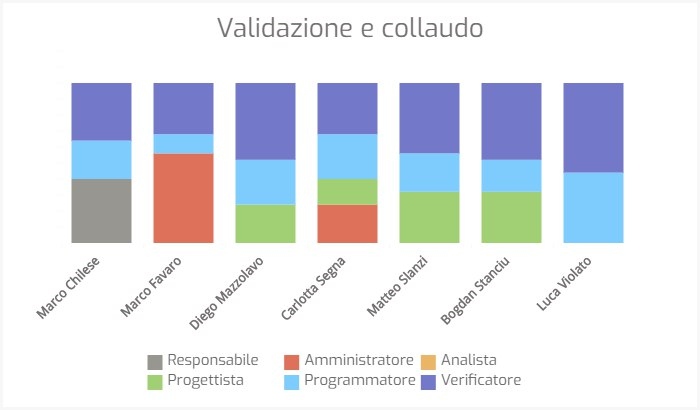
\includegraphics[width=1\linewidth]{./images/Bar_validazione_collaudo.png}
	\caption{Grafico suddivisione ore per persona nel periodo di Validazione e collaudo}
	\label{fig:grafico suddivione ruoli periodo di Validazione e collaudo}
\end{figure}

\begin{longtable}{| C{.30\textwidth}| C{.15\textwidth}| C{.20\textwidth}|}
	\hline
	\textbf{Ruolo} & \textbf{Ore} & \textbf{Costo in \euro} \\
	\hline 
	Responsabile & 10 & \EUR{300.00} \\
	\hline
	Amministratore & 20 & \EUR{400.00}\\
	\hline
	Analista & 0 & \EUR{0.00} \\
	\hline
	Progettista & 23 & \EUR{506.00} \\
	\hline
	Programmatore & 48 & \EUR{720.00} \\
	\hline
	Verificatore & 74 & \EUR{1110.00} \\
	\hline
	\textbf{Totale} & 175 & \EUR{3036.00}\\ 
	\hline
	
	\caption{Distribuzione oraria del periodo di Validazione e collaudo}
	\label{Distribuzione oraria del periodo di Validazione e collaudo}
\end{longtable}

Il seguente grafico dà una rappresentazione visiva della suddivisione nei ruoli:
\begin{figure}[H]
	\centering
	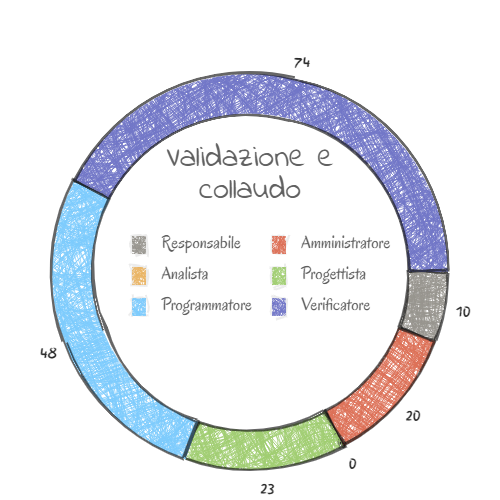
\includegraphics[width=0.8\linewidth]{./images/torta_validazione_col.png}
	\caption{Grafico suddivisione ore per persona nel periodo di Validazione e collaudo}
	\label{fig:grafico suddivione ruoli periodo di Validazione e collaudo}
\end{figure}

\newpage

\subsection{Totale ore rendicontate}
\subsubsection{Prospetto orario}

Le ore di seguito riportate sono da considerarsi a carico del committente, che non includono le ore della prima fase:

\begin{longtable}{|C{.30\textwidth}|C{.06\textwidth}|C{.06\textwidth}|C{.06\textwidth} | C{.06\textwidth}| C{.06\textwidth} | C{.06\textwidth} | C{.10\textwidth} |}
\hline
\textbf{Nome} & \textbf{RE} & \textbf{AM} & \textbf{AN} & \textbf{PJ} & \textbf{PR} & \textbf{VE} & \textbf{Totale}\\
\hline 
Marco Chilese & 10 & 16 & 13 & 25 & 31 & 28 & 123\\
\hline
Marco Favaro & 16 & 14 & 15 & 15 & 24 & 39 & 123\\
\hline
Diego Mazzalovo & 8 & 8 & 7 & 34 & 41 & 25 & 123\\
\hline
Carlotta Segna & - & 19 & 5 & 24 & 46 & 29 & 123\\
\hline
Matteo Slanzi & 10 & - & 17 & 28 & 39 & 29 & 123\\
\hline
Bodgan Stanciu & 7 & 8 & 17 & 34 & 25 & 32 & 123\\
\hline
Luca Violato & 15 & 7 & 7 & 23 & 32 & 39 & 123 \\
\hline

\caption{Distribuzione oraria delle ore rendicontate}
\label{Distribuzione oraria delle ore rendicontate}
\end{longtable}

Il seguente grafico dà una visione grafica della suddivisione dei ruoli per il periodo di Risanamento criticità:\begin{figure}[H]
	\centering
  		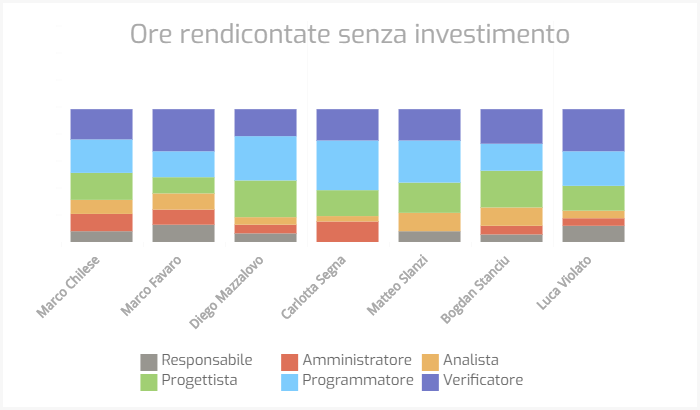
\includegraphics[width=1\linewidth]{./images/totale_ore_rendicontate_senza_investimento.png}
  		\caption{Grafico suddivisione ore nei ruoli senza investimento.}
  		\label{fig:grafico suddivione ruoli}
\end{figure}


\subsubsection{Prospetto economico}
\begin{longtable}{| C{.30\textwidth}| C{.15\textwidth}| C{.20\textwidth}|}
\hline
\textbf{Ruolo} & \textbf{Ore} & \textbf{Costo in \euro} \\
\hline
Responsabile & 66 & \EUR{1980.00} \\
\hline
Amministratore & 72 & \EUR{1440.00} \\
\hline
Analista & 81 & \EUR{2025.00} \\
\hline
Progettista & 183 & \EUR{4026.00}\\
\hline 
Programmatore & 238 & \EUR{3570.00} \\
\hline
Verificatore & 221 & \EUR{3315.00} \\
\hline 
\textbf{Totale} & 861 & \EUR{16356.00}\\
\hline

\caption{Distribuzione oraria a carico del committente}
\label{Distribuzione oraria a carico del committente}
\end{longtable}

\begin{figure}[H]
	\centering
  		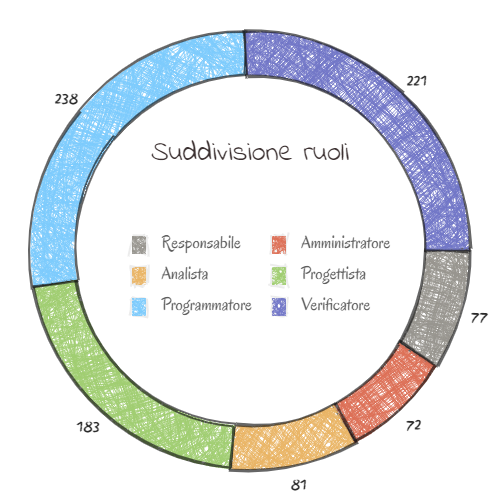
\includegraphics[width=0.8\linewidth]{./images/torta_sr.png}
  		\caption{Grafico suddivisione ore nei ruoli senza investimento.}
  		\label{fig:grafico suddivione ruoli}
\end{figure}



\subsection{Totale ore con investimento}
\subsubsection{Prospetto orario}


\begin{longtable}{|C{.30\textwidth}|C{.06\textwidth}|C{.06\textwidth}|C{.06\textwidth} | C{.06\textwidth}| C{.06\textwidth} | C{.06\textwidth} | C{.10\textwidth} |}
\hline
\textbf{Nome} & \textbf{RE} & \textbf{AM} & \textbf{AN} & \textbf{PJ} & \textbf{PR} & \textbf{VE} & \textbf{Totale}\\
\hline 
Marco Chilese & 10 & 16 & 23 & 25 & 31 & 43 & 148\\
\hline
Marco Favaro & 16 & 14 & 29 & 15 & 24 & 50 & 148\\
\hline
Diego Mazzalovo & 8 & 8 & 25 & 34 & 41 & 32 & 148\\
\hline
Carlotta Segna & 11 & 19 & 10 & 24 & 46 & 38 & 148\\
\hline
Matteo Slanzi & 10 & 8 & 27 & 28 & 39 & 36 & 148\\
\hline
Bodgan Stanciu & 22 & 8 & 24 & 34 & 25 & 35 & 148\\
\hline
Luca Violato & 15 & 22 & 12 & 23 & 32 & 44 & 148 \\
\hline


\caption{Distribuzione oraria delle ore con investimento}
\label{Distribuzione oraria delle ore con investimento}
\end{longtable}

\begin{figure}[H]
	\centering
  		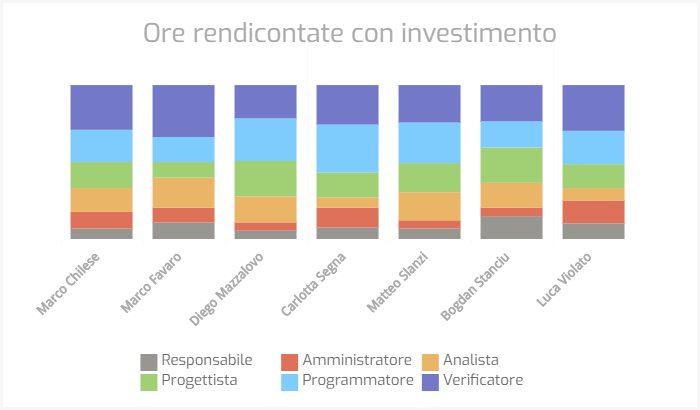
\includegraphics[width=1\linewidth]{./images/ore_rendicontate_con_investimento.png}
  		\caption{Grafico suddivisione ore nei ruoli con investimento.}
  		\label{fig:grafico suddivione ruoli con investimento}
\end{figure}

\subsubsection{Prospetto economico}

\begin{longtable}{| C{.30\textwidth}| C{.15\textwidth}| C{.20\textwidth}|}
\hline
\textbf{Ruolo} & \textbf{Ore} & \textbf{Costo in \euro} \\
\hline 
Responsabile & 92 & \EUR{2760.00}\\
\hline
Amministratore & 95 & \EUR{1900.00} \\
\hline
Analista & 150 & \EUR{3750.00} \\
\hline 
Progettista & 183 & \EUR{4026.00}\\
\hline
Programmatore & 238 & \EUR{3570.00} \\
\hline
Verificatore & 221 & \EUR{3315.00} \\
\hline
\textbf{Totale} & 979 & \EUR{19321.00} \\
\hline
\caption{Distribuzione oraria nei ruoli con investimento}
\label{Distribuzione oraria ruoli con investimento}
\end{longtable}

\begin{figure}[H]
	\centering
  		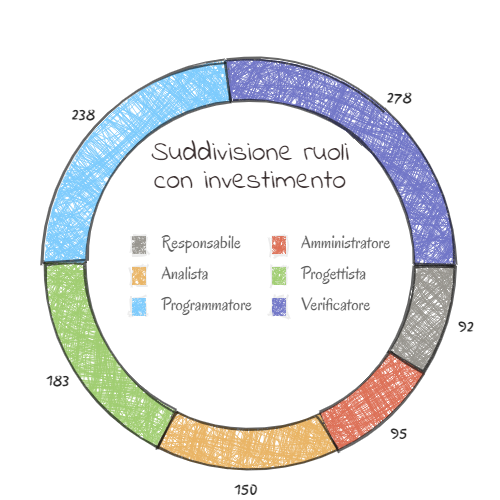
\includegraphics[width=0.8\linewidth]{./images/torta_srci.png}
  		\caption{Grafico suddivisione ore nei ruoli con investimento.}
  		\label{fig:grafico suddivione ruoli con investimento}
\end{figure}



